\begin{figure}
    \centering
    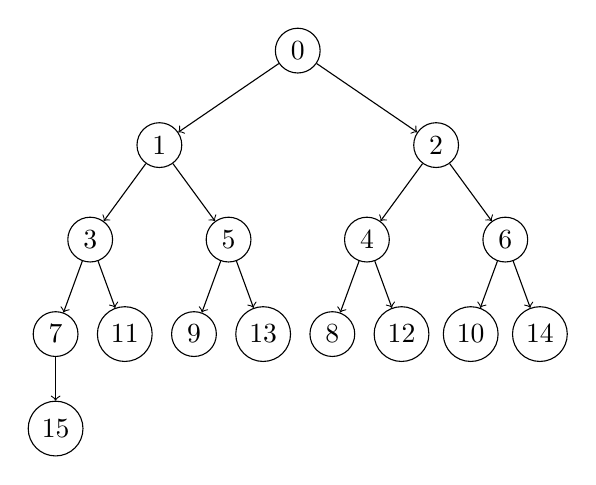
\begin{tikzpicture} [every node/.style = {shape=circle, draw, align=center}, inner sep=1mm, level distance=12mm]
        \tikzstyle{level 1}=[sibling distance=10em]
        \tikzstyle{level 2}=[sibling distance=5em]
        \tikzstyle{level 3}=[sibling distance=2.5em]
        \node {0}
        child [->] { node {1}
                child { node {3}
                        child {node {7} child {node {15}}}
                        child {node {11}}
                    }
                child { node {5}
                        child {node {9}}
                        child {node {13}}
                    }
            }
        child [->] { node {2}
                child { node {4}
                        child {node {8}}
                        child {node {12}}
                    }
                child { node {6}
                        child {node {10}}
                        child {node {14}}
                    }
            };


    \end{tikzpicture}
    \caption{16 process binary tree broadcast.}
    \label{fig:graph-bin-tree}
\end{figure}
